\section{DiemBFT协议}

DiemBFT协议的目标是按顺序提交块。该协议在一系列轮次中运作。在每一轮中,一位领导者提出一个新的区块。验证节点将投票发送给下一轮的领导者。当投票达到法定人数时,下一轮的领导者将形成法定人数证书(QC),并将其嵌入下一个提案中。验证节点也可能在一轮超时时放弃。这可能会导致在没有获得QC的情况下过渡到下一轮,在这种情况下,验证节点形成或观察当前轮的超时证书(TC),通过视图更改机制进入下一轮。事实上,进入r + 1轮需要观察r轮的QC或TC。下一轮的领导者面临如何扩展其知道的当前块树的选择。在DiemBFT中,领导者总是从证书树的最高分支延伸直接子区块。其优点是块树具有统一的结构,每个区块都有一个直接父区块的 QC。作为DiemBFT链接方法的结果,DiemBFT中的块树可能包含在轮数中有间隙的链。

轮次信息被显式地包含在块中,判断何时提交的逻辑是很简单的:它需要一个2-链,其中包含连续的轮次数,其最后一个后代已被认证。当两个不间断的轮次完成时,“2-链”的头部(由已形成QC的两个连续回合组成)将被提交。参见图1中的插图。

以新提交的块结尾的整个分支变为已提交状态。图2显示了一个块树,包括一个未提交的分叉。分叉可能是由于各种原因造成的,比如恶意领导者、消息丢失等。例如,该图显示了一个拜占庭领导者在区块 k 处分叉了该链,导致一条未提交的链被放弃。k 块对其父块使用与左叉相同的 QC。在所描述的场景中,k块被提交,而左分支被丢弃。请注意,正如我们稍后所解释的,我们的安全规则保证提交的分支永远不会被丢弃。

\begin{figure}[htbp]
    \centering
    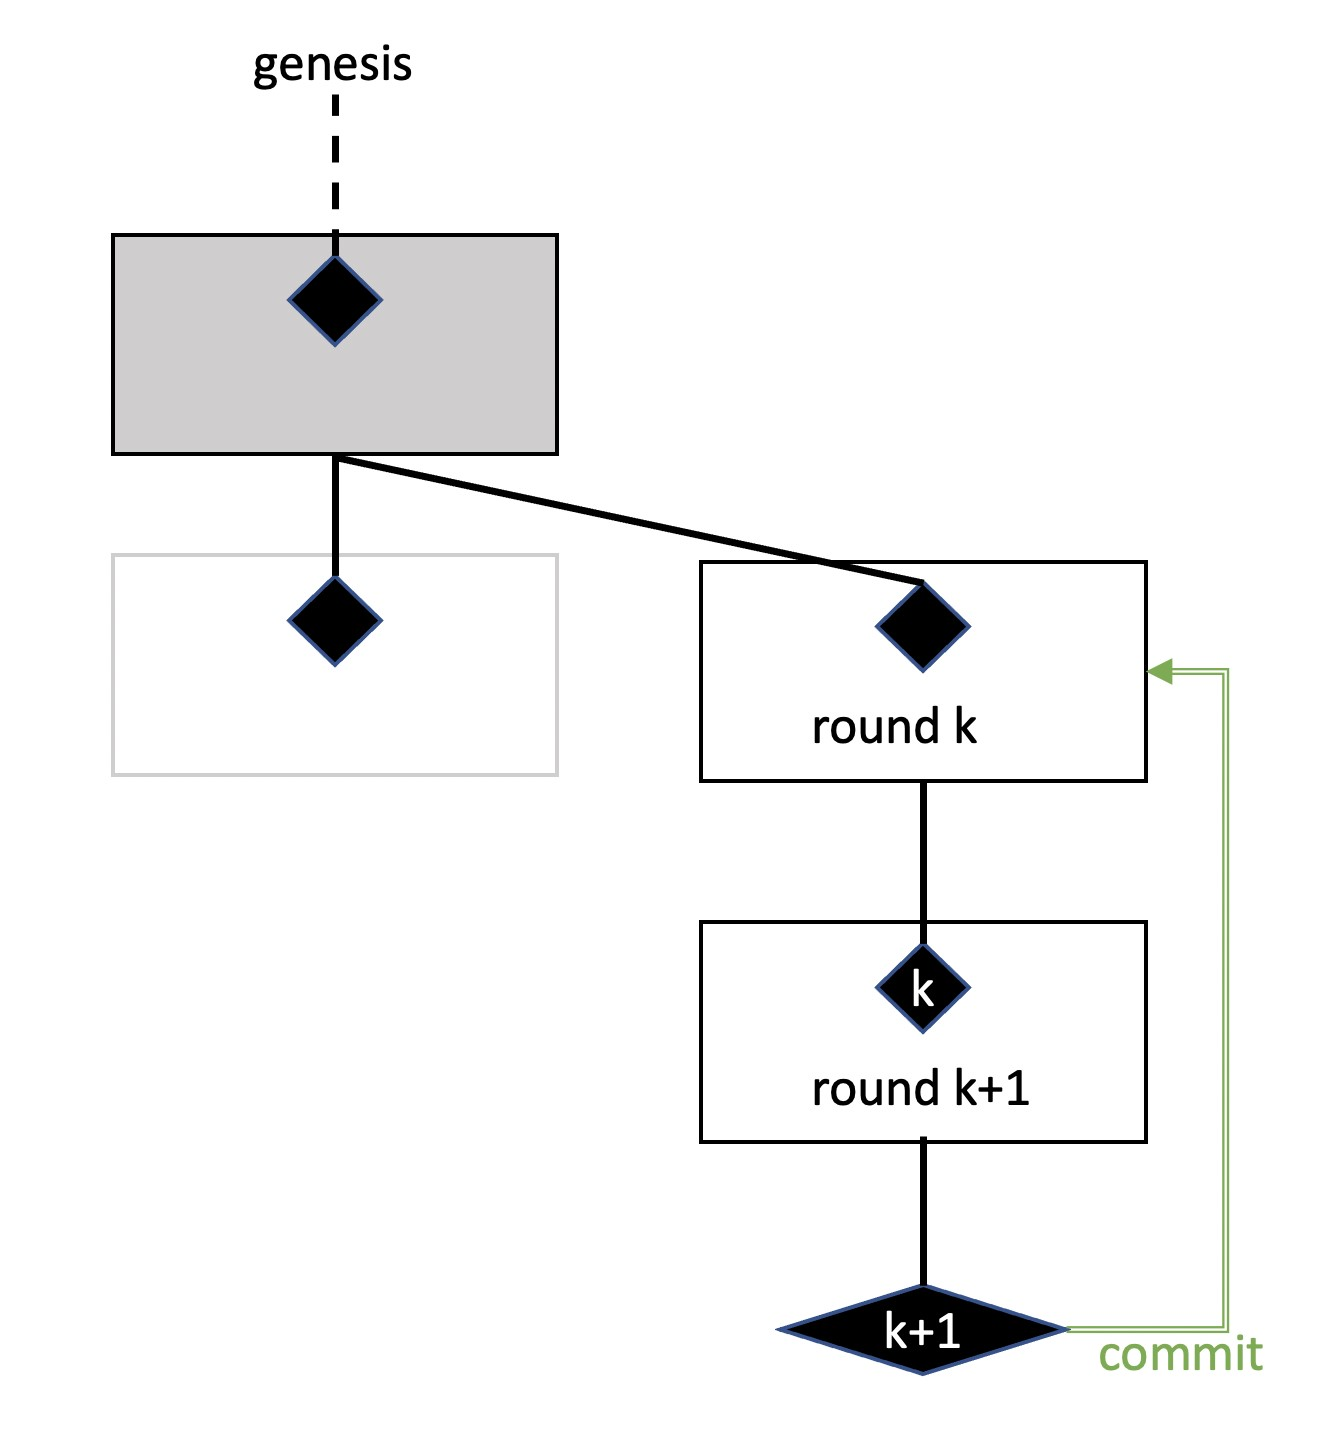
\includegraphics[width=6cm]{figures/image2.jpg}
    \caption{提交之前和之后在块树中待处理的提案(块)}
    \label{image2}
\end{figure}

DiemBFT 通过由两个要素组成的简单投票规则保证只有一个分叉被提交:首先,验证节点在严格递增的轮次中投票。其次,每个区块必须包含上一轮的 QC 或 TC。 如果上一轮的结果是 TC,那么验证节点会检查新领导者的提议是否可以安全扩展。该检查包括查看来自不同节点的 2f+1 个 highest\_qc\_round(验证节点投票支持的块中包含的最高 QC)的 TC。 如果新提案扩展了这些 highest\_qc\_round 中的最高值,这可以证明更高一轮的任何内容都不能提交(否则至少有人会报告更高的最高 qc\_round)。 考虑图 3 中描述的场景,其中 k + 4 QC 是在第 k + 3 轮提交块时形成的。在未来的轮次中,不可能形成一个允许扩展低于 k + 3 的 QC 的 TC。

我们继续详细描述DiemBFT协议,详细说明实现中的数据结构和模块。实现分为以下几个模块:
\begin{itemize}
    \item 首先是一个主模块(第3.1节),它是胶水、调度消息和计时器事件处理程序。
    \item 一个账本(第3.2节)模块,用于存储本地可分叉的推测性账本状态。它为SMR服务提供接口,并连接到更高级别的逻辑(执行)。
    \item 生成提案块的块树(第3.3节)模块。它通过投票和QC对等待提交的区块树进行跟踪。
    \item 实施核心共识安全规则的安全模块(第3.4节)。安全:私有部分控制私钥,并处理签名的生成和验证。它保持最低状态,并可由安全的硬件组件保护。
    \item 一个起搏器(第3.5节)模块,用于维持活动性并推进循环。它为安全提供了“听觉节拍”。
    \item MemPool(第3.6节)模块,在生成提案时向领导提供交易。
    \item 最后,一个LeaderElection(第3.7节)模块将轮次映射到领导者,并在静态碰撞故障下实现最佳领导者利用率,同时在拜占庭式故障下保持链质量。
\end{itemize}

\begin{figure}[htbp]
    \centering
    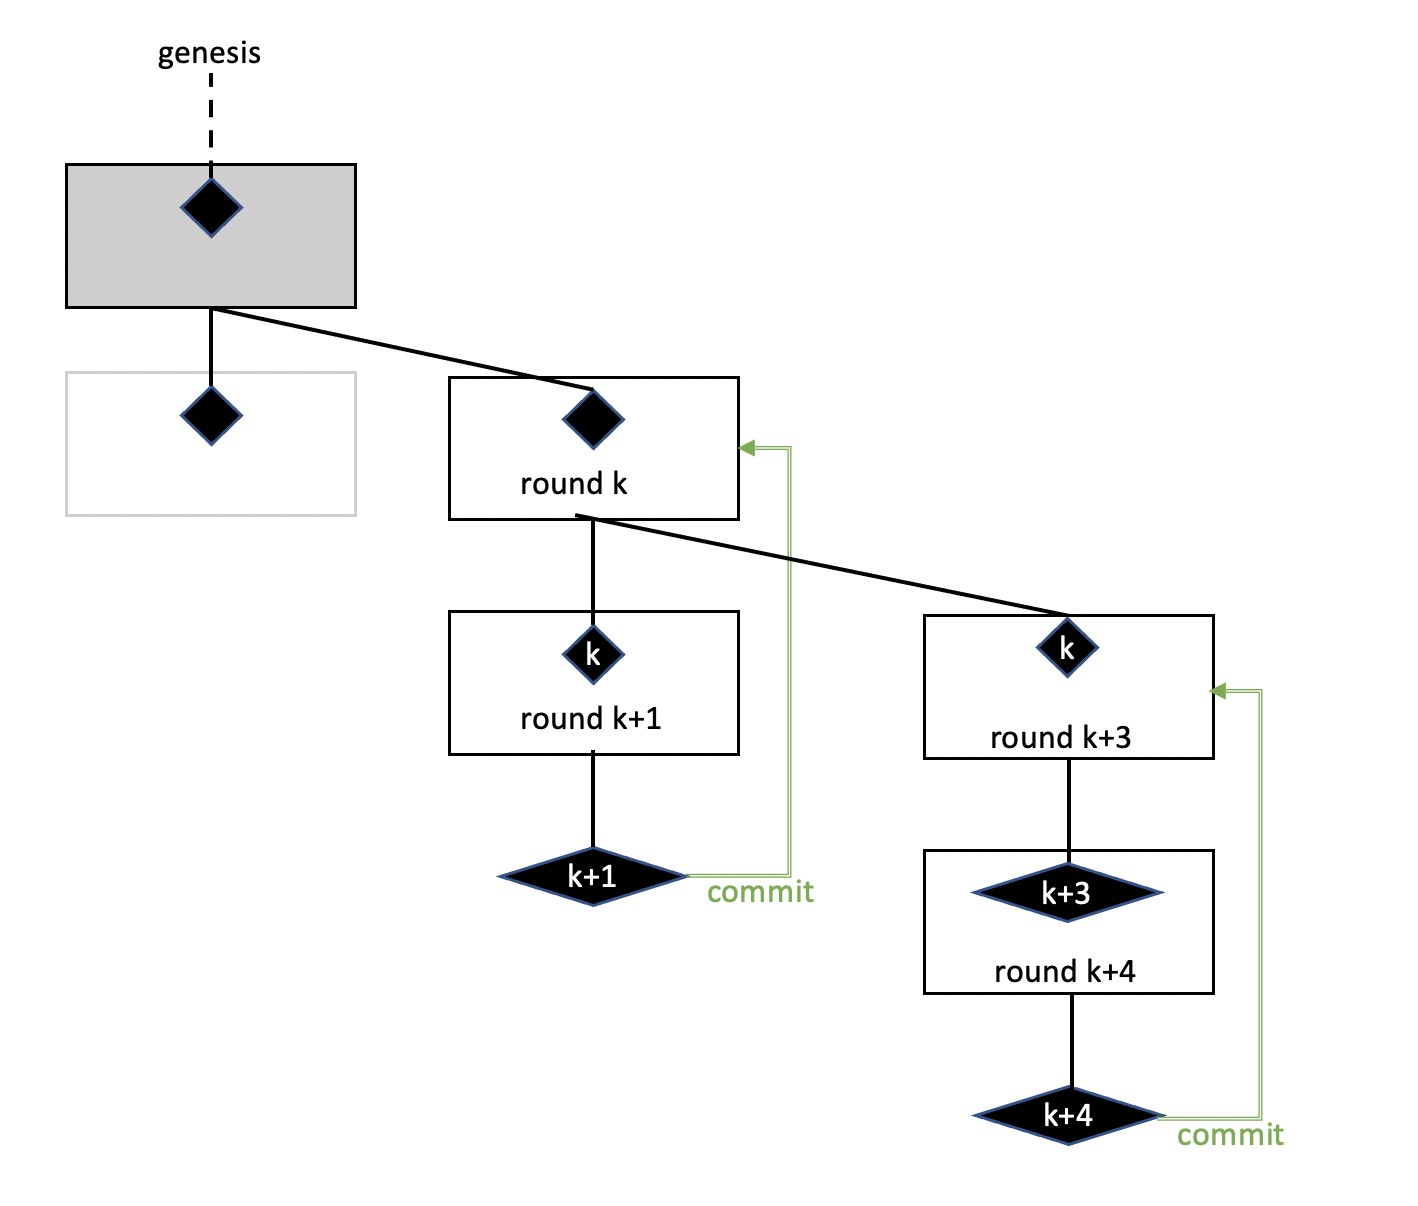
\includegraphics[width=6cm]{figures/image3.jpg}
    \caption{提交的区块形成一个单调递增的链}
    \label{image3}
\end{figure}

第4节给出了形式正确性证明。

\subsection{主模块}

\begin{figure}[htbp]
    \centering
    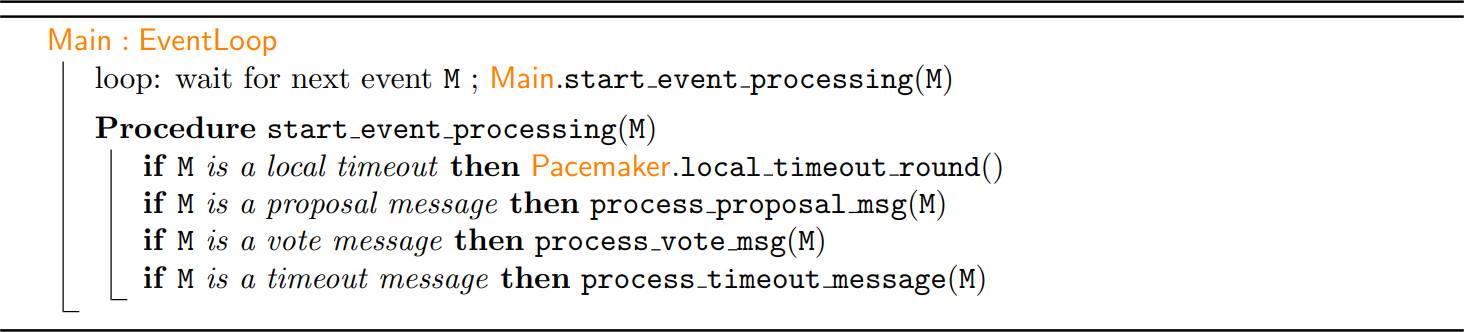
\includegraphics[width=12cm]{figures/code1.png}
\end{figure}

DiemBFT的主要模块是一个事件处理循环,它调用适当的处理程序来处理消息和事件。它处理以下事件:提议消息、投票消息、远程超时消息和本地超时。

\begin{figure}[H]
    \centering
    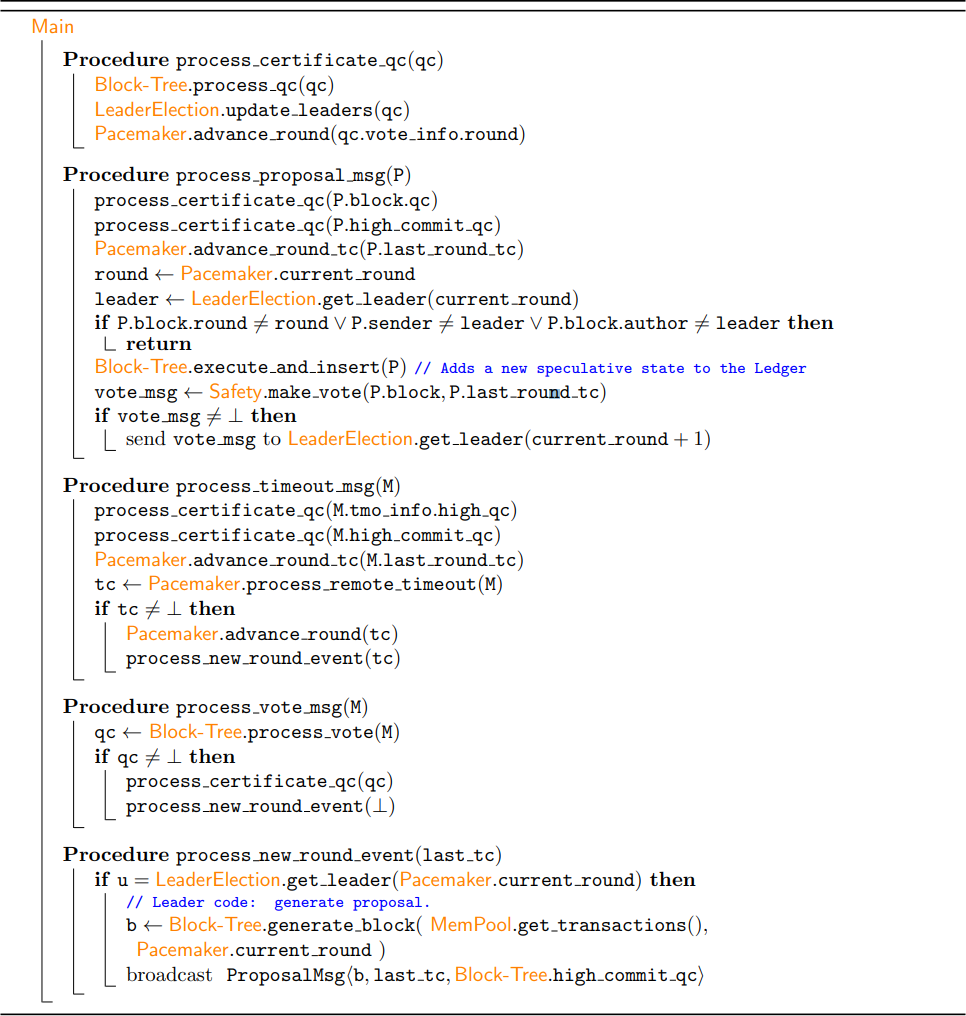
\includegraphics[width=12cm]{figures/code1-1.png}
\end{figure}

% \begin{algorithm}[htb]
%     \caption{题目}
%     \label{alg:Framwork}
%     \begin{algorithmic}
%         \State Fuck You
%     \end{algorithmic}
%   \end{algorithm}
  

% \begin{algorithm}
%     \caption{title}%标题
%     \label{alg1}%标签
%     \begin{algorithmic}
%         \State Main: EventLoop

%         loop: wait for next event M; Main.start\_event\_processing(M)

%         \State Procedure start\_event\_processing(M)

%             \If{M is a local timeout}  
%             \State Pacemaker.local\_timeout\_round()
%             % \EndIf

%             if M is a proposal message then process\_proposal\_msg(M)

%             if M is a vote message then process\_vote\_msg(M)

%             if M is a timeout message then process\_timeout\_message(M)
      
%     \end{algorithmic}
% \end{algorithm}

\subsection{账本模块}

最终,Diem区块链的目标是维护一个可编程资源数据库,该数据库由DiemBFT共识核心负责复制。数据库由抽象账本状态表示。从DiemBFT的角度来看,账本持久化存储和执行虚拟机的大部分实现细节(应用了改变账本状态的交易)特意保持不透明和通用性;特别是,Move 事务执行的细节超出了本手稿的范围。

每个DiemBFT验证节点的本地账本模块充当辅助账本存储的网关。它维护一个本地未决(可能产生分支)推测性账本状态,该状态扩展了最后提交的状态。推测树被验证节点保存在本地的内存中,直到一个分支被提交。它提供了一个从等待提交的区块到推测性账本状态的映射。

Ledger.speculate(prev\_block\_id, block\_id, txns) API 推测性地在前一个区块状态上执行一个交易区块,并返回一个新的账本状态id。推测性执行可能会将账本状态分支为多个(冲突的)分叉,形成一个推测状态树。最终,一个分支被共识引擎所提交。Ledger.commit() API 将提交的分支导出到账本持久存储,并抛弃了本地中从提交状态的祖先那里分叉的推测分支。

重要的是要强调,账本支持投机执行,以便正确处理执行中的潜在不确定性。如果我们构建的系统只是对事务进行排序,以便将它们传递到执行层,那么我们就不需要维护推测状态树,因为VM只会执行提交的事务。然而,这样的系统将无法容忍任何不确定性(例如,由于硬件缺陷):在DiemBFT没有意识到这一点的情况下,验证节点会出现分歧。因此,DiemBFT不仅仅是对事务进行排序:它确保投票证明了事务及其执行结果。应该有至少 2f + 1 个诚实的验证节点到达相同的状态,以便为一个交易块形成一个 QC。

DiemBFT 只需要账本模块提供上述的基本API。

\begin{figure}[htbp]
    \centering
    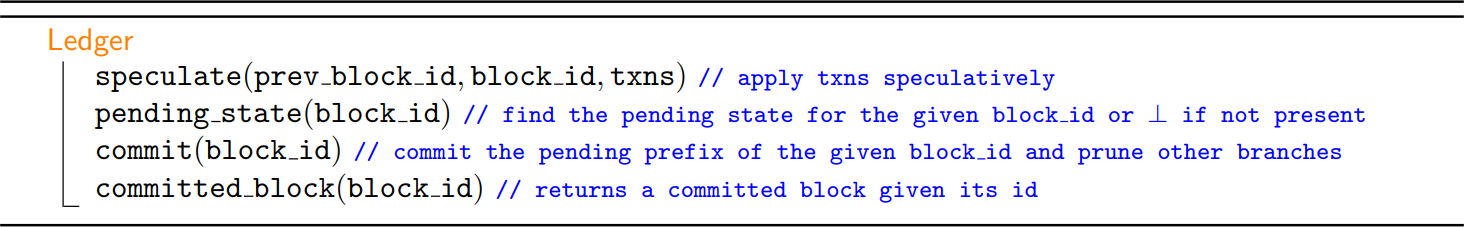
\includegraphics[width=12cm]{figures/code2.png}
\end{figure}

\subsection{块树模块}

块树模块由两种核心数据类型组成,验证协议围绕这两种数据类型构建:块和投票。从投票中派生的另一种数据类型是法定人数证书(QC),它由块上的一组投票组成。下文起搏器模块中描述了一种仅与超时和轮次推进有关的额外数据类型。块树模块跟踪所有待决区块的树以及它们收到的投票。

\begin{figure}[htbp]
    \centering
    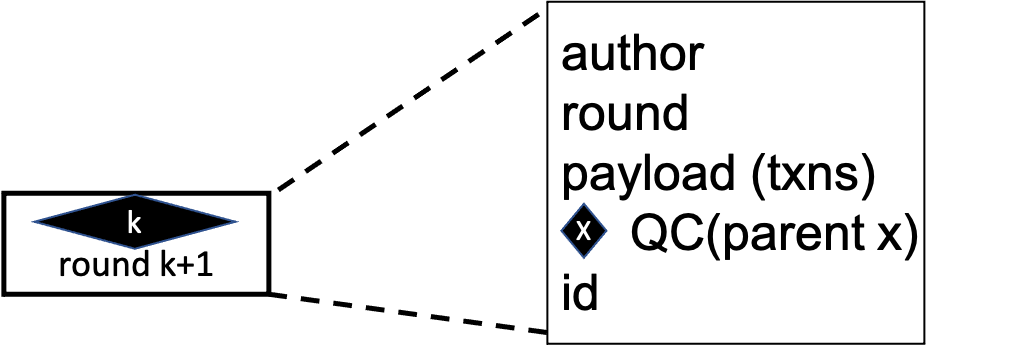
\includegraphics[width=6cm]{figures/image5.png}
    \caption{块树中的一个块}
    \label{image5}
\end{figure}

\subsubsection{块}

共识协议用于形成账本交易协议的核心数据结构是块。每个块包含一组提议的账本交易,以及用于形成共识决策的附加信息。每个区块b(已知的genesis区块P0除外)通过 b.qc 链接到父区块,b.qc 是一个法定人数证书(qc),由父区块的法定投票数组成。通过这种方式,待提交的块形成了一个以 P0 为根的提议块树。

块b的投票信息VoteInfo必须同时包含块id和推测的执行状态exec\_state\_id,以保证确定的执行结果。此外,VoteInfo保存了b的父节点的id和轮次。为方便起见,保留此信息,允许从单个块推断提交状态而不获取其祖先块。此外,投票消息还包括LedgerCommitInfo,这是一种推断的已提交账本状态,由commit\_state\_id标识。当区块的QC导致其父区块提交时,区块上的法定人数投票也用于证明新的已提交账本状态。

LedgerCommitInfo有两个用途。首先,它包括commit\_state\_id,可以将其作为历史证明提供给客户端(实际上,commit\_state\_id 可以是覆盖账本历史的 Merkle树根的哈希)。只要客户能够验证给定的账本状态是否由2f +1参与者签名,他们就不需要知道共识协议的细节。其次,LedgerCommitInfo包含VoteInfo的哈希。这个哈希对客户端来说是不透明的,只被共识参与者使用。因此,签署投票消息的验证节点对潜在的LedgerCommitInfo(由账本存储作为提交证明)和嵌入在其投票块中的QC(用于运行共识协议)进行验证。请注意,块的id包括节点签名的摘要,因此每一轮投票的投票者集合都是被唯一确定的。

\begin{figure}[H]
    \centering
    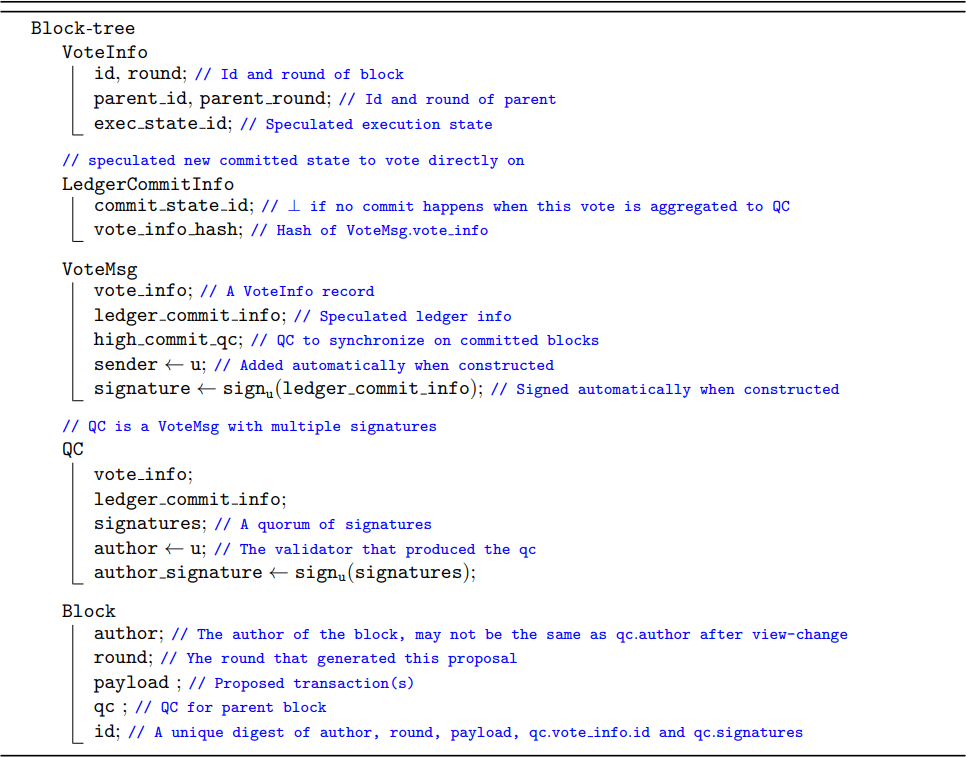
\includegraphics[width=12cm]{figures/code11.png}
\end{figure}

例如,考虑在第 k 轮中的提议 b,在第 k -1 轮中具有父 b0。 如果验证节点决定投票给 b,它会签署一个 LedgerCommitInfo,其中包括 b0 的潜在提交以及 b 上的 VoteInfo 的哈希。

块树模块跟踪未在待定投票中形成 QC 的投票。 pendingblocktree 是一个推测性的块树,类似于 Ledger 构建一个推测性的状态树。 实际上,pendingblocktree 中的块和 Ledger 中的块之间存在 1:1 的映射关系。 当一个新块被添加到pendingblocktree时,它也会被添加到Ledger中。 投票基于分类帐提交信息的哈希在 PendingVotes 中聚合。 一旦有 2f + 1 票,他们就组成了一个 QC。

该算法在 high\_qc 中维护已知的最高认证块,在形成新QC或作为提案的一部分接收新QC时对其进行更新。新提案延伸自验证节点本地已知的最高认证块。

\begin{figure}[H]
    \centering
    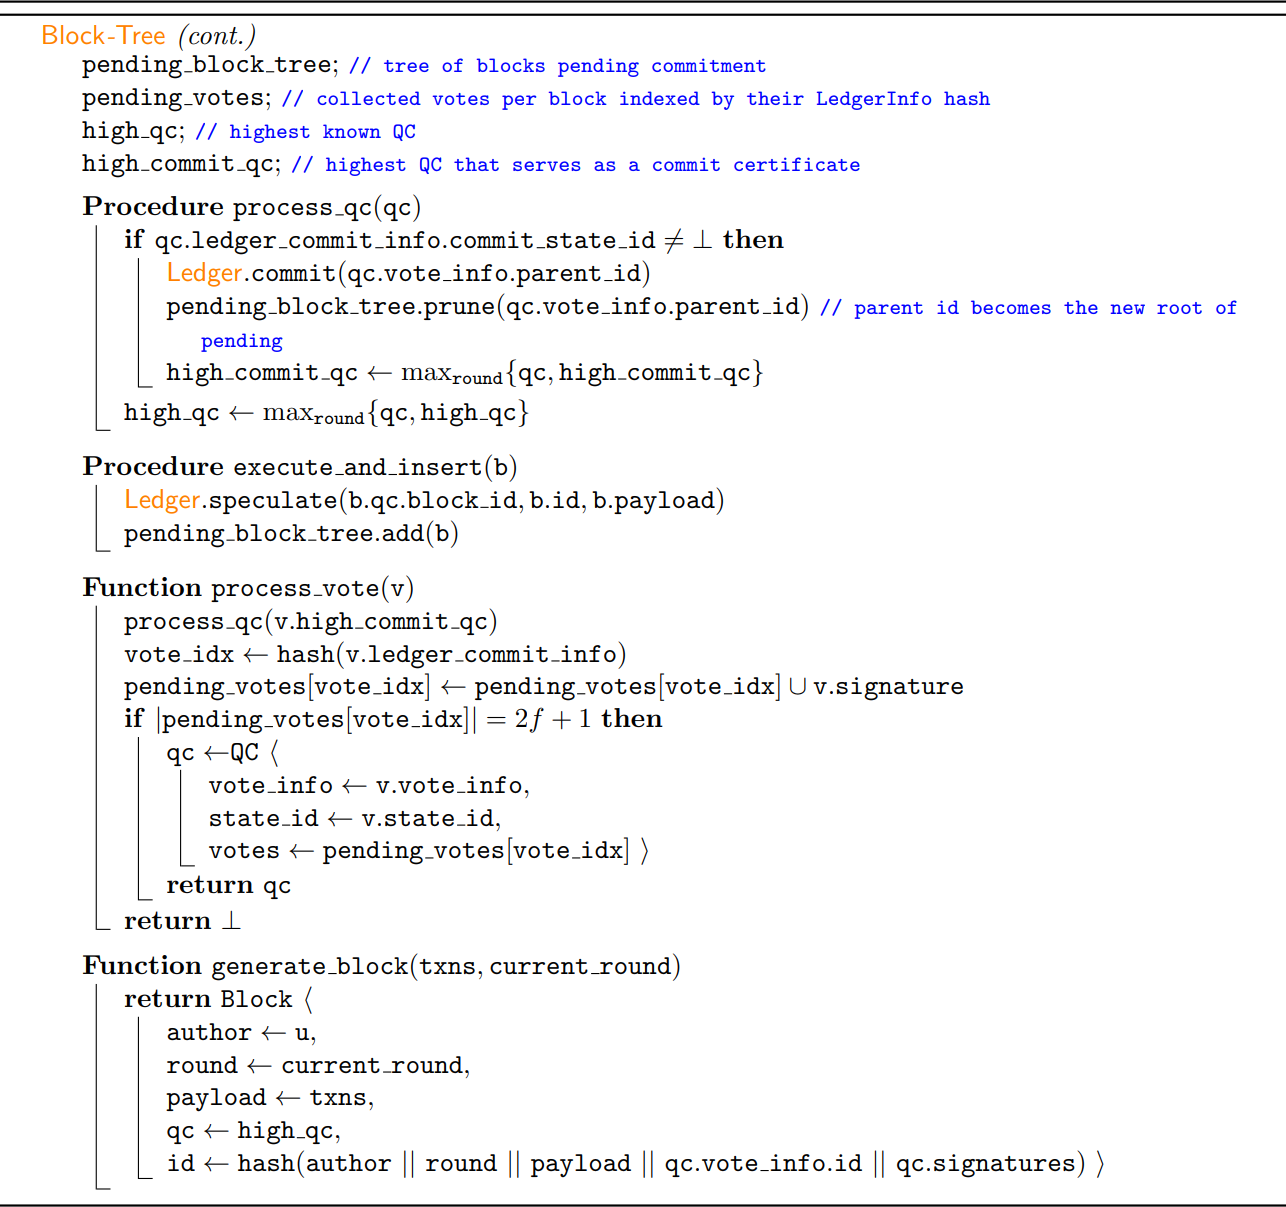
\includegraphics[width=12cm]{figures/code4.png}
\end{figure}

\subsubsection{剩余的消息和证书类型}

超时证书是另一种类型的证书,用于在由于某种原因无法形成正常投票的QC时推进一轮投票。除了VoteMsg,还有另外两种类型的消息TimeoutMsg和ProposalMsg。

\begin{figure}[H]
    \centering
    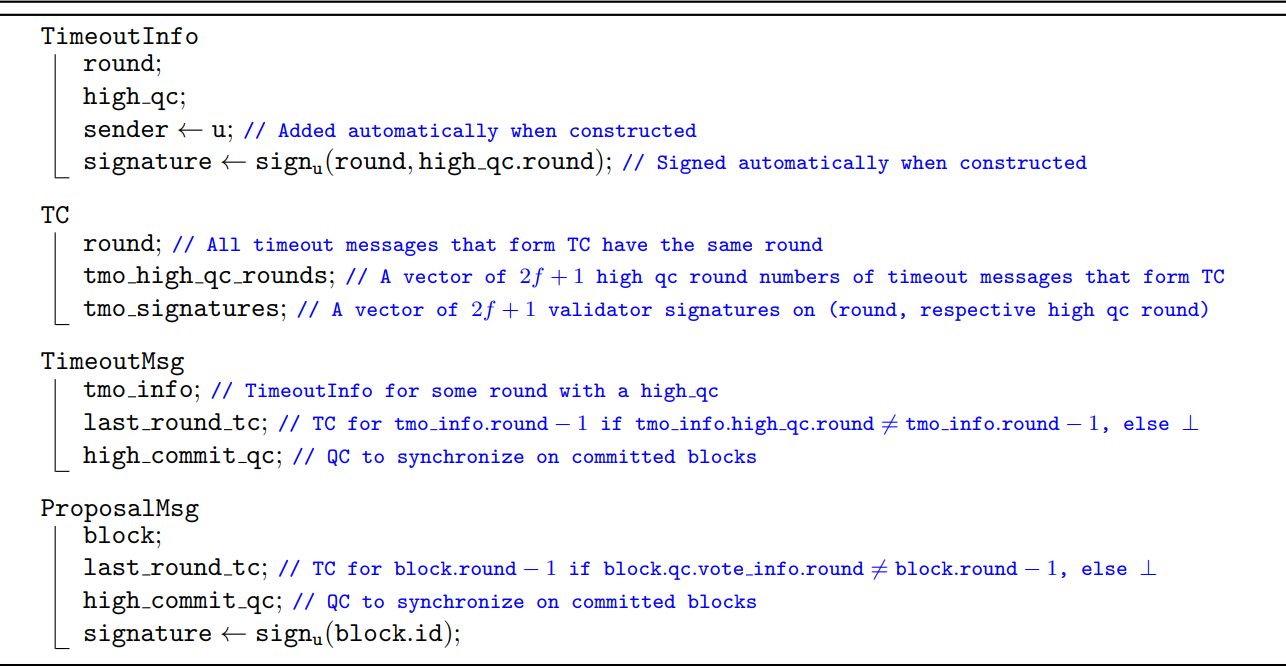
\includegraphics[width=12cm]{figures/code5.png}
\end{figure}

如果超时消息中包含的 tmo\_info.high\_qc 或提案消息中包含的 block.qc(父 QC)包含第 r - 1 轮的 TC 作为last\_round\_tc,则轮 r 的超时消息或提案消息是格式良好的 ,分别不是来自第 r - 1 轮(否则, last\_round\_tc 是不相关的,并且按照惯例设置为 ⊥)。 格式不正确的消息会被诚实的验证节点丢弃,而诚实的验证节点总是会生成格式正确的超时和提议消息。

\subsection{安全模块}

在DiemBFT中,当一个块成为一个连续的2-链的头部时,它就被提交,比如该块的轮紧跟在其父块的轮之后。这将在commit\_state\_id\_candidate 函数中进行检查。

为了能够在受信任的硬件上部署安全模块,DiemBFT仅维护以下两个计数器:(i)highest\_vote\_round 保留最后一轮投票的轮次,以及(ii)highest\_vote\_round 保留验证节点投票的区块中包含的最高QC的轮次。

在收到提案b(一个区块)时,验证节点仅在b轮的轮次高于其最后一轮投票时才投票给b。此外,验证节点借助safe\_to\_vote谓词进行判断,该谓词封装了投票安全性逻辑。

完整安全模块的逻辑如下所示。首先,我们描述只能从安全模块内部访问的私有成员和接口。

\begin{figure}[H]
    \centering
    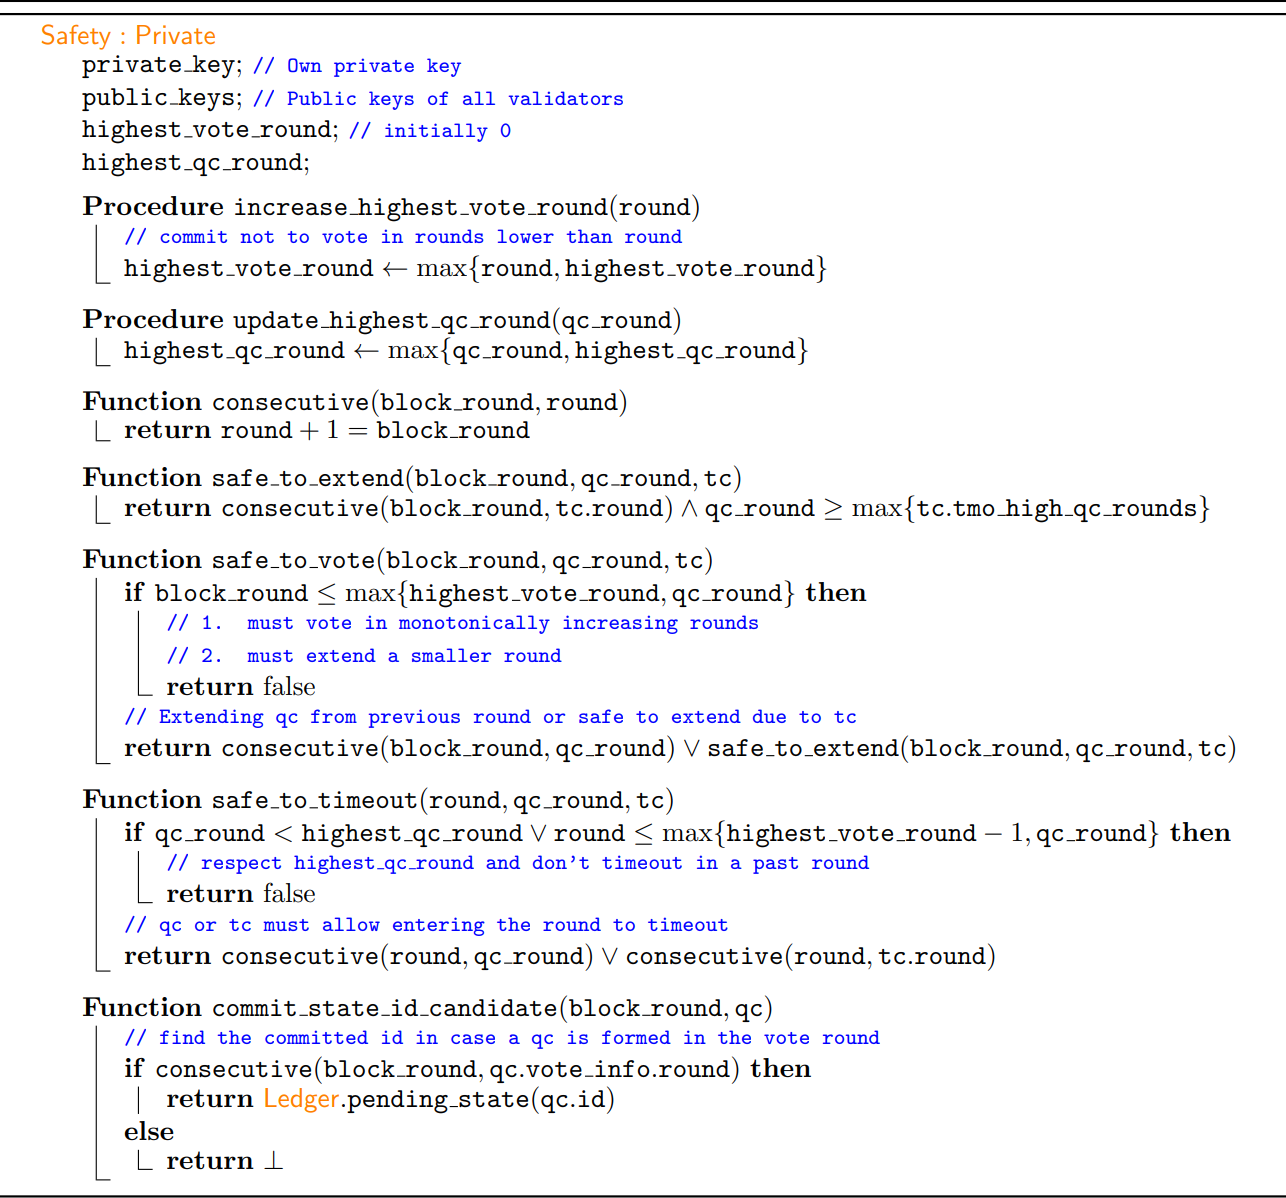
\includegraphics[width=12cm]{figures/code6.png}
\end{figure}

其他模块使用下面描述的安全模块的公共接口来构造两种类型的投票(VoteMsg和 TimeoutMsg)。因此,任何有效的投票都由安全模块进行签名,该模块拥有私钥。我们还假设,在这些函数的开头调用valid\_signatures会检查格式,并检查为构造投票而提供的所有参数上的签名(使用其他验证节点的公钥)。系统的其他部分也会检查消息的格式和签名(例如,当第一次收到任何类型的消息时),但为了防止安全性受损,验证节点需要自己进行一层签名检查。

\begin{figure}[H]
    \centering
    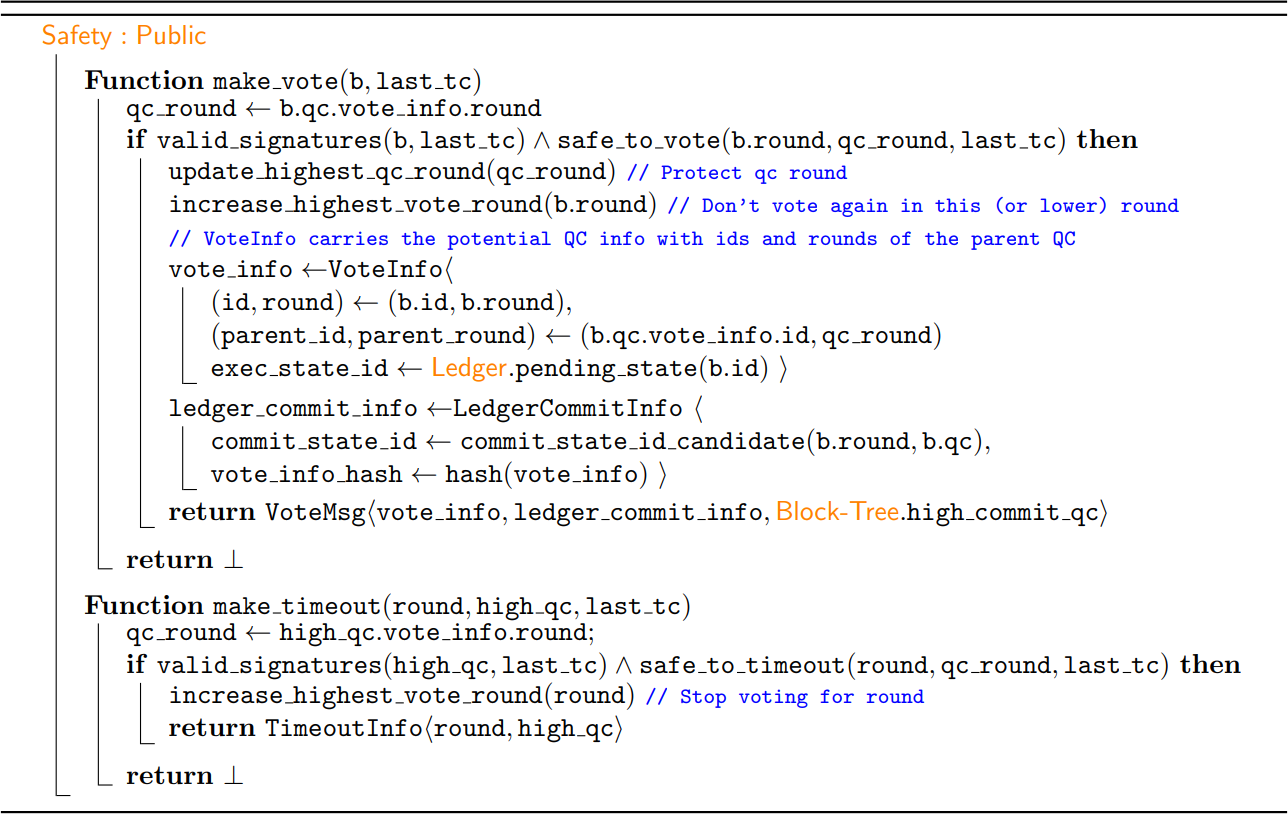
\includegraphics[width=12cm]{figures/code7.png}
\end{figure}


请注意,安全模块不需要外部依赖,只根据提案及其QC的轮次与潜在提交信息生成投票。这有助于验证安全性,并允许分离安全模块,以便在TCB内执行。

\subsection{起搏器模块}

轮次的推进由一个名为起搏器的模块控制。起搏器记录投票和时间。在一条“正常路径”中,每个验证节点的起搏器模块使用领导者提案中的QC来推进轮次。在“恢复路径”中,心脏起搏器观察到一轮中没有进展,并根据超时证书推进一轮。

当本地轮超时时,起搏器会广播TimeoutMsg通知。此消息包含 high\_qc 并由安全模块签名,安全模块验证最高 QC 轮次不高于 high\_qc 轮次。这对于确保后来的领导者不能在最后一个提交的块之下分叉是很重要的。此外,high\_qc 信息有助于领导者和慢速节点保持最新状态。在发送TimeoutMsg消息后,验证节点会增加他们的最高投票轮次,以确保他们不会在这轮投票中投票。	

当验证节点接收到r轮的f + 1超时消息时,如果它还没有超时,它将在第r轮超时。当接收到2f + 1个超时消息时,验证节点可以形成一个TC并推进一轮。


\begin{figure}[H]
    \centering
    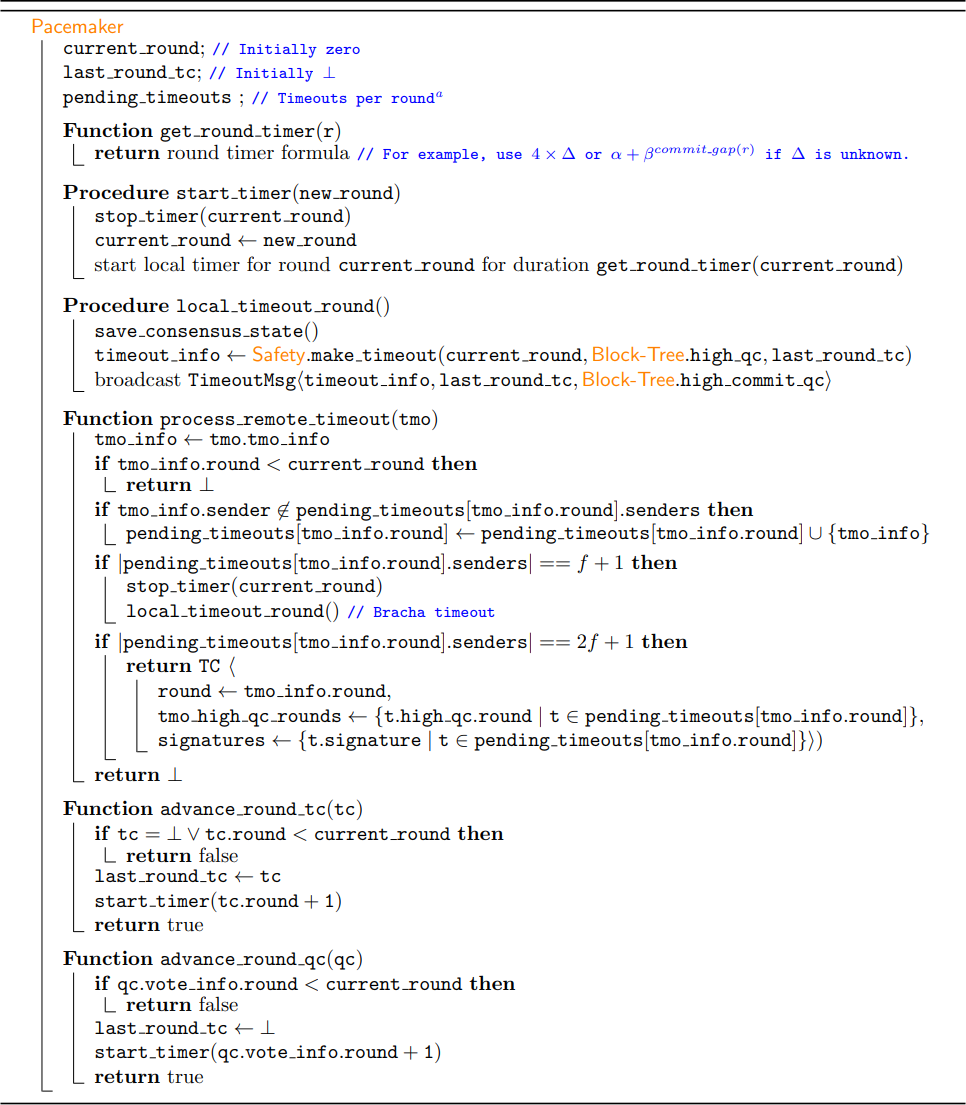
\includegraphics[width=12cm]{figures/code8.png}
\end{figure}

因此,如果一个验证节点已经形成了TC,那么所有其他诚实的验证节点将在两个网络传输 延迟内做同样的事情。

\subsection{内存池抽象模块}

我们假设有一个MemPool模块,它提供交易来作为块的负载。

\begin{figure}[H]
    \centering
    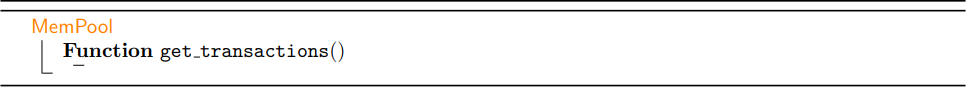
\includegraphics[width=12cm]{figures/code9.png}
\end{figure}

\subsection{主节点选举模块}

PBFT 等经典的一致性算法,领导者在被怀疑出现崩溃或拜占庭式的故障之前会稳定的持有领导身份。然而,在区块链协议中,这不是一个合适的策略,区块链协议需要确保诚实的验证节点提交的方案得到提交,即链质量。一种解决方案是每轮轮换领导者,让每个诚实的验证节点都有平等的机会提出一个值。然而,这导致崩溃的验证节点在恢复之前继续当选为领导者。

为了解决这个问题,我们提出了一种基于声誉的领导者选举机制,根据之前的积极参与程度确定当选领导者的资格时。然而,如果天真地这样做,这种机制可能会让对手控制领导者的选择,或者让诚实的验证节点对领导者的身份产生分歧。

\begin{figure}[H]
    \centering
    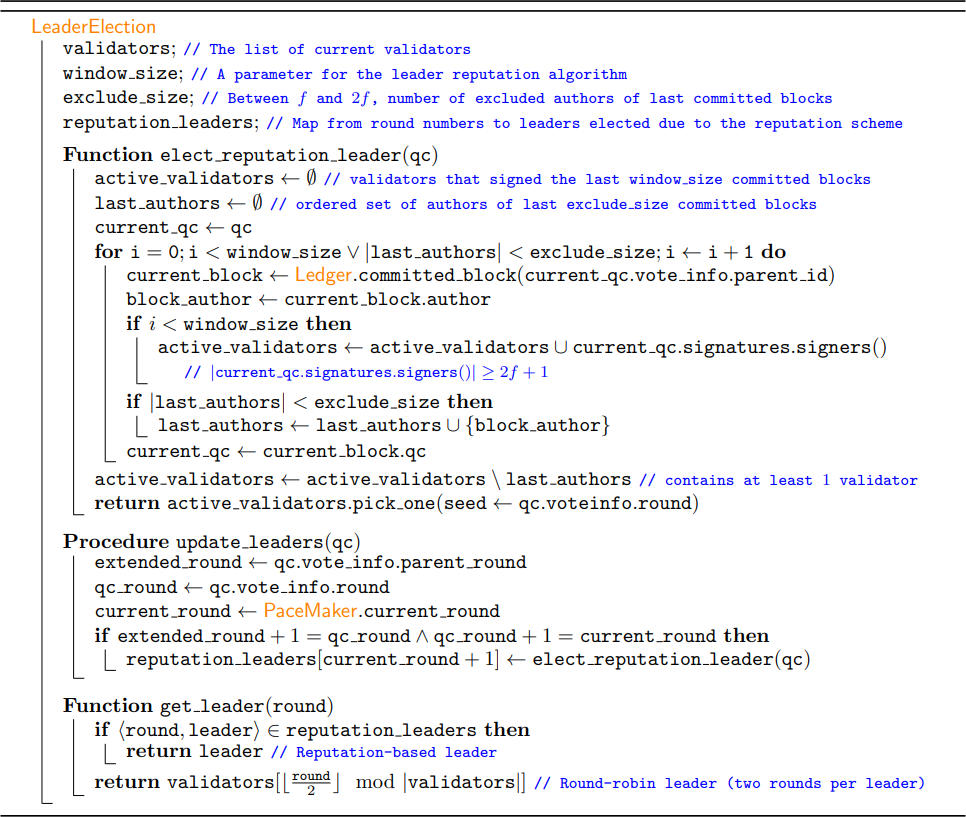
\includegraphics[width=12cm]{figures/code10.png}
\end{figure}

在 DiemBFT 中,验证节点有两条路径来确定领导者。 如果诚实的验证节点在第 r 轮获得一个带有 r-2 轮提交的 QC 的块,那么领导者声誉方案使用提交信息来确定第 r+1 轮的领导者。特别的,领导者声誉方案使用 QC 签名者信息来确定活跃验证节点的集合,然后(出于链质量目的)排除 exclude\_size 个最新已提交区块的领导者,并从剩余集合中确定性地选择领导者。否则,如果验证节点在第 r 轮没有提交第 r-2 轮(由于拜占庭行为、崩溃或消息延迟),它使用轮询来确定第 r+1 轮的领导者。 这意味着不同的副本可能不会遵循相同的路径,这会导致它们在下一个领导者上存在分歧。 然而,正如我们稍后证明的那样,这只会在 GST 之后发生几次。

领导者选举机制的目的是通过在领导者轮换中检测并排除崩溃的验证节点,减少崩溃故障对共识延迟的影响。从形式上讲,对于没有拜占庭式失败的执行,我们要求:

\begin{itemize}
    \item t-领导者利用率:考虑一次没有拜占庭验证节点的运行。然后,在GST之后,最多有t轮会出现诚实的验证节点不同意领导者,或者他们的领导者崩溃的情况。
\end{itemize}

上述属性优化了领导者因崩溃而失败的更大可能性的场景。然而,该协议必须能够抵御最坏情况下的对手,包括拜占庭验证节点。为此,我们要求在最坏的拜占庭条件下保持以下特性:

\begin{itemize}
    \item 活跃度:GST之后会提交无限多个区块。
    \item t-链质量:在t个提交块的任何窗口中,至少有一个是由诚实的领导者提出的。我们在第4.2 节中证明了上述保证以及响应范围。
\end{itemize}

实际上,我们可能希望缓慢的验证节点也有机会成为领导者。这可以通过包括不在活动验证节点∪最新块作者集合中的验证节点来实现,因为他们被选为领导者,而相对活跃的同行而言,他们的权重较低。这引入了领导者利用率的权衡。